Nas figuras \ref{fig:peppers:hilbert} e \ref{fig:watch:hilbert}, podemos ver que as curvas de Hilbert causam um contraste maior na imagem. Isso é um indicativo que os erros não estão sendo distribuídos corretamente, provavelmente devido à algum problema de implementação.

\begin{figure}[H]
    \centering
    \begin{subfigure}{0.33\textwidth}
    \centering
    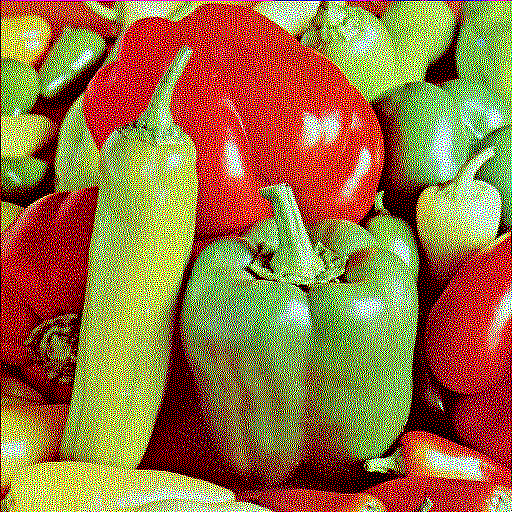
\includegraphics[width=4.4cm]{resultados/dists/peppers_floyd.png}
    \caption{Floyd e Steinberg.}
    \label{fig:peppers:floyd}
\end{subfigure}%
\begin{subfigure}{0.33\textwidth}
    \centering
    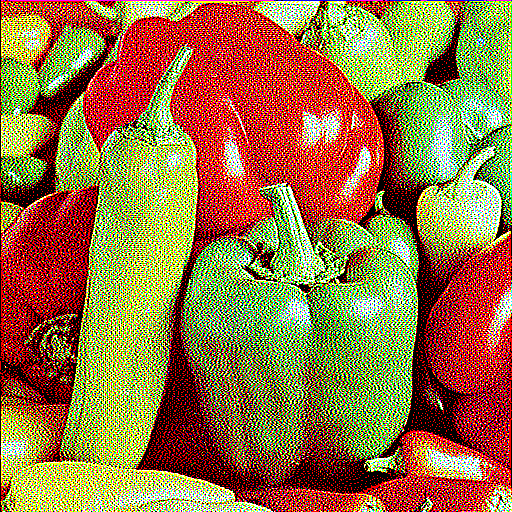
\includegraphics[width=4.4cm]{resultados/dists/peppers_stevenson.png}
    \caption{Stevenson e Arci.}
    \label{fig:peppers:stevenson}
\end{subfigure}%
\begin{subfigure}{0.33\textwidth}
    \centering
    \includegraphics[width=4.4cm]{resultados/dists/peppers_burkes.png}
    \caption{Burkes.}
    \label{fig:peppers:burkes}
\end{subfigure}\\[8pt]
\begin{subfigure}{0.33\textwidth}
    \centering
    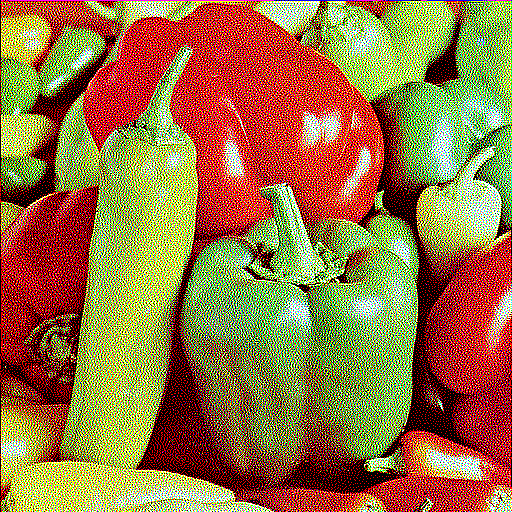
\includegraphics[width=4.4cm]{resultados/dists/peppers_sierra.png}
    \caption{Sierra.}
    \label{fig:peppers:sierra}
\end{subfigure}%
\begin{subfigure}{0.33\textwidth}
    \centering
    \includegraphics[width=4.4cm]{resultados/dists/peppers_stucki.png}
    \caption{Stucki.}
    \label{fig:peppers:stucki}
\end{subfigure}%
\begin{subfigure}{0.33\textwidth}
    \centering
    \includegraphics[width=4.4cm]{resultados/dists/peppers_jarvis.png}
    \caption{Jarvis, Judice e Ninke.}
    \label{fig:peppers:jarvis}
\end{subfigure}
    \caption{Aplicação das quatro varreduras na \texttt{peppers.png}.}
    \label{fig:extra:peppers}
\end{figure}

Já as curvas em espiral funcionam como esperado, entretanto aparecem, em ambas as figuras \ref{fig:peppers:espiral} e \ref{fig:watch:espiral}, artefatos nas diagonais da imagem, onde ocorre a rotação da matriz de distribuição de erros.

\begin{figure}[H]
    \centering
    \begin{subfigure}{0.33\textwidth}
    \centering
    \includegraphics[width=4.4cm]{resultados/extra/watch_unidirecional.png}
    \caption{Unidirecional}
    \label{fig:watch:unidirecional}
\end{subfigure}%
\begin{subfigure}{0.33\textwidth}
    \centering
    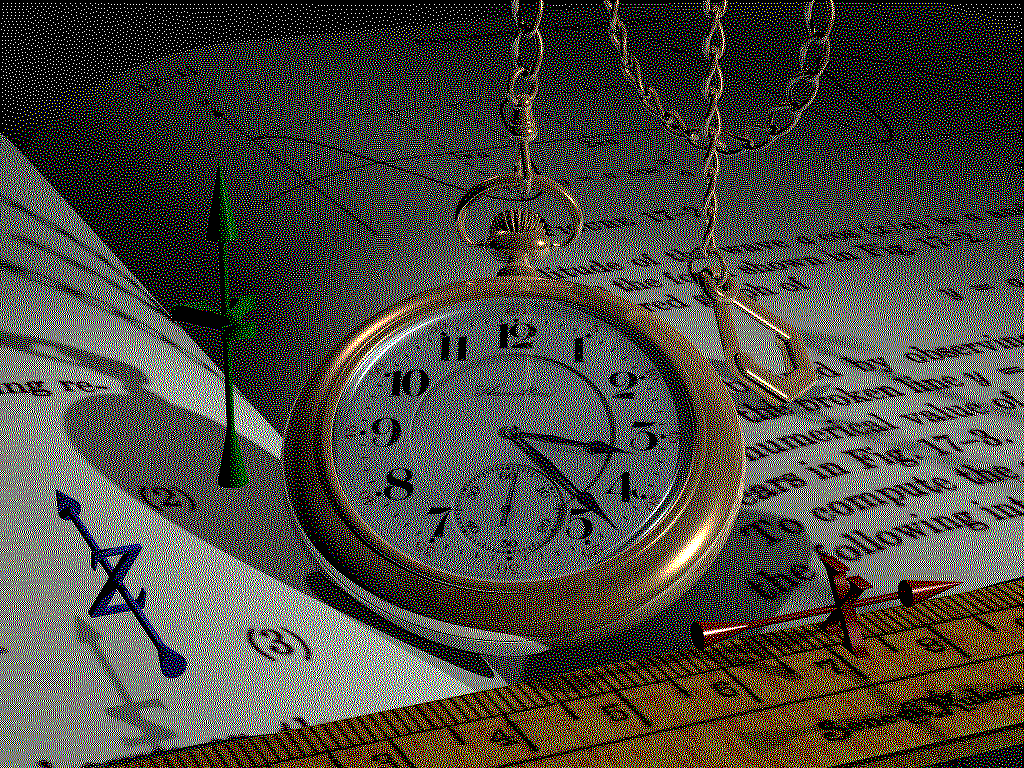
\includegraphics[width=4.4cm]{resultados/extra/watch_alternada.png}
    \caption{Alternada}
    \label{fig:watch:alternada}
\end{subfigure}\\[8pt]
\begin{subfigure}{0.33\textwidth}
    \centering
    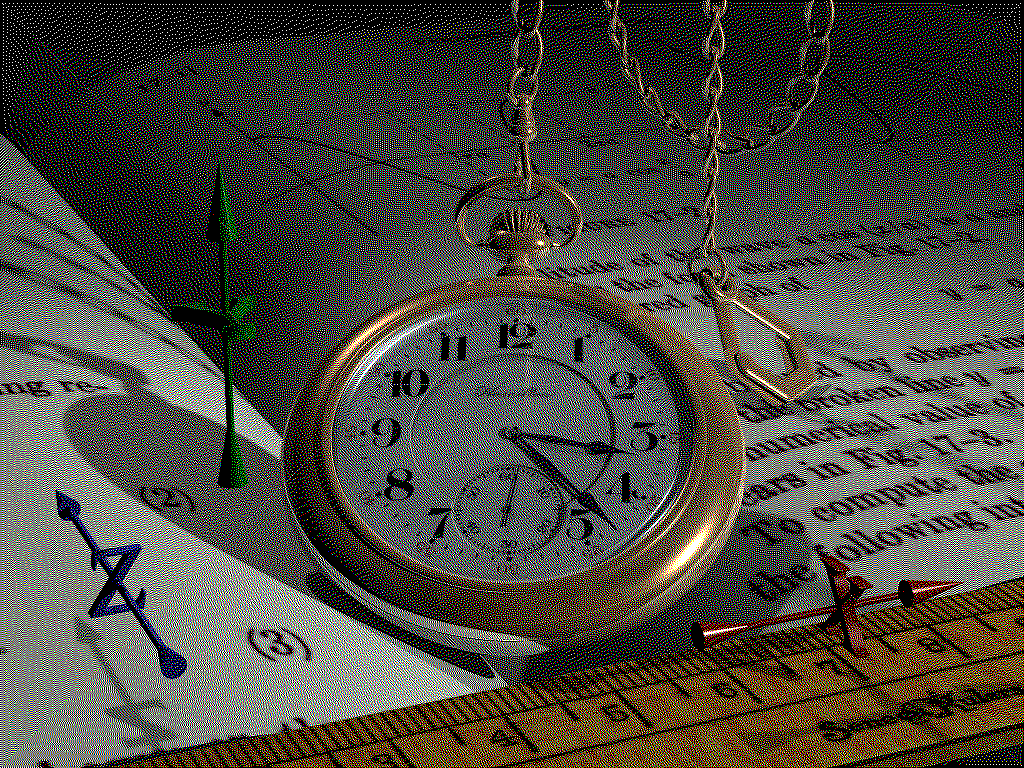
\includegraphics[width=4.4cm]{resultados/extra/watch_espiral.png}
    \caption{Espiral}
    \label{fig:watch:espiral}
\end{subfigure}%
\begin{subfigure}{0.33\textwidth}
    \centering
    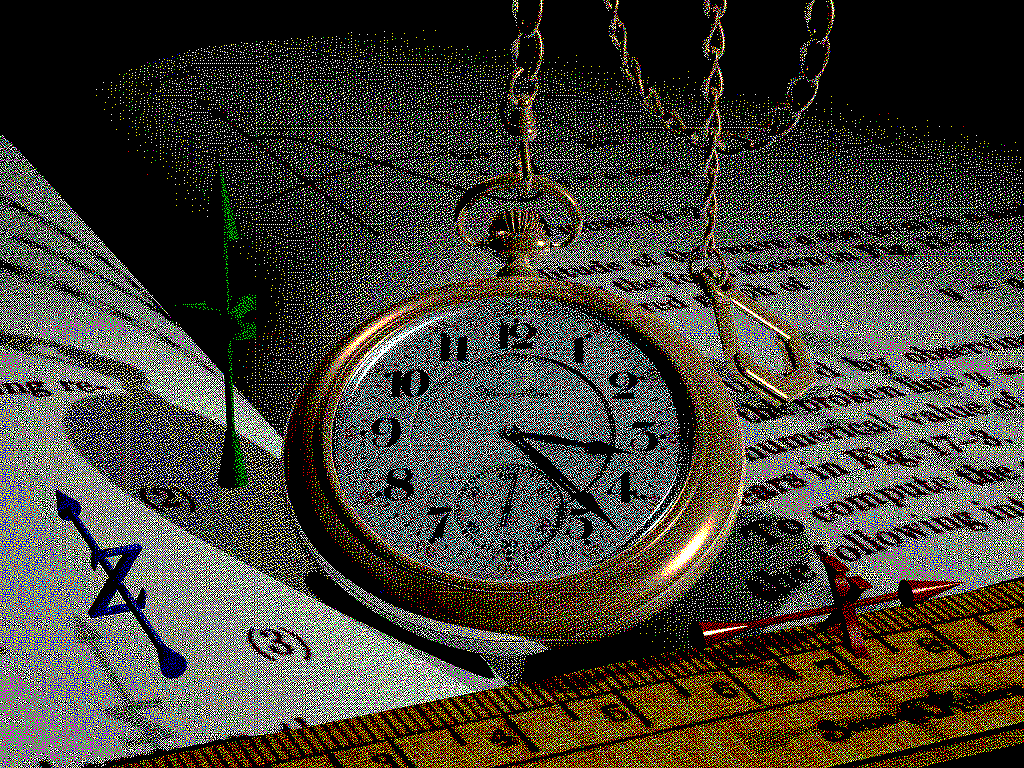
\includegraphics[width=4.4cm]{resultados/extra/watch_hilbert.png}
    \caption{Hilbert}
    \label{fig:watch:hilbert}
\end{subfigure}
    \caption{Aplicação das qautro varreduras na \texttt{watch.png}.}
    \label{fig:extra:watch}
\end{figure}
